\section{Mapping}
I mapping study sono effettuati per avere un quadro completo
delle conoscenze attualmente disponibili in una certa area di ricerca. Il mapping viene eseguito attraverso il conteggio dei contributori in relazione alle categorie che sono state approfondite. Un mapping ha lo scopo di approfondire quali argomenti
sono stati trattati e dov’è possibile reperire tali informazioni. Essendo però un processo sistematico, condivide molte delle metodologie di una revisione sistematica della letteratura. Quello che però fa discostare un mapping da una
\emph{systematic review} sono gli obiettivi finali: durante una revisione sistematica si punta a sintetizzare delle evidenze in un determinato campo di analisi, nello studio delle
mappature sistematiche l’obiettivo è piuttosto definire un'area di ricerca.
Per definire un mapping sistematico, \textbf{Petersen et al}.[4] propongono di seguire la seguente linea guida:
\begin{itemize}
	\item Domande di ricerca: Individuare le domande per le quali ricercare una risposta. Tali domande guideranno tutto lo studio;
	\item Ricerca della documentazione: Individuare le parole chiave più opportune da formulare per effettuare la fase di ricerca;
	\item Criteri di inclusione/esclusione: Individuare dei criteri per scartare risultati non inerenti allo studio;
	\item Valutazione della qualità: Valutare i risultati in base alla loro qualità;
	\item Estrazione dei dati: Sintetizzare i risultati in base alle domande di ricerca che sono state poste;
	\item Analisi e classificazione: Visualizzare le informazioni di ogni item di ricerca e raggrupparle in base a caratteristiche comuni;
	\item Validazione: Descrivere eventuali minacce dello studio condotto e valutare la ripetibilità dello studio.
\end{itemize}
\section{Mapping study flaky test}
\subsection{Domande di ricerca}
La prima fase per effettuare il mapping study legato alla problematica dei \emph{flaky test} è stata l’individuazione delle domande di ricerca. Sono state quindi poste
le seguenti domande:
\begin{enumerate}[start=0,label={(\bfseries RQ\arabic*):}]
	\item È stato rilasciato un dataset?
	\item Hanno lavorato anche su progetti closed source?
	\item Viene detto in che linguaggio di programmazione sono scritti i progetti utilizzati?
	\item Viene descritto che tipo di sistema di building utilizzano?
	\item Sono state definite le tecniche che hanno utilizzato per sviluppare il dataset?
	\item Vengono definite quali sono le root cause più frequenti che sono state individuate?
	\item Viene definito che metodo empirico hanno utilizzato per individuare le root cause?
	\item Viene detto a chi è indirizzata questa ricerca?
	\item In che anno è stata pubblicata la ricerca?
\end{enumerate}

Dopo aver individuato le domande di ricerca, si è passati a identificare le stringhe da utilizzare. Per poterle individuare è stato seguito il modello PICO (\emph{Population, Intervention, Comparison and Outcomes}) sviluppato da \textbf{Kitchenham} e \emph{Charters} che ha portato ai seguenti risultati:
\begin{itemize}
	\item \emph{Population}: Ingegneri del software;
	\item \emph{Intervention}: Continuous integration;
	\item \emph{Comparison}: Strategie per identificare i flaky test e comparare la costruzione di dataset per progetti open source e closed source;
	\item \emph{Outcomes}: comprendere lo stato dell’arte e le cose che sono state fatte.
\end{itemize}

Tramite questo modello, sono state individuate le seguenti keywords: \emph{“Software testing”, “Continuous Integration”, “Flaky test”, “dataset”, “open source”, “closed source”}.

Successivamente sono stati individuati tre tra i più importanti databases per la raccolta di dati in letteratura, ovvero \textbf{IEEE}, \textbf{ACM} e \textbf{Scopus} e sono state formulate le seguenti query.
\newpage
\begin{table}[h!]
	\centering
	\scalebox{0.7}{\begin{tabular}{|l|l|}
		\hline
		\textbf{Database} & \textbf{Search}                                                                                                                                                                                                                                                                                                                                                                                                                                                                                                         \\ \hline
		IEEE              & \begin{tabular}[c]{@{}l@{}}((("flaky" OR "flakiness" OR "test pass and fail" \\ OR "non deterministic") AND "test" AND \\ ("SE" OR "software engineering" OR\\  "computer science")) AND \\ ((("dataset" OR "database")OR\\  ("project open source" OR \\ "close* source" OR "source code"))OR\\  ("build* system*" OR \\ "maven" OR "gradle" OR\\  "continuous integration" OR\\  "integration")OR ("root cause" AND \\ ("detect*" OR "improve*"))))\end{tabular}                                                      \\ \hline
		ACM               & \begin{tabular}[c]{@{}l@{}}((("flaky" OR "flakiness" OR\\  "test pass and fail" OR\\  "non deterministic test*") AND\\  "test" AND\\  ("SE" OR "software engineering" OR\\  "computer science")) AND\\  ((("dataset" OR "database" OR\\  "db")OR ("project open source" OR\\  "close* source" OR "source code")) OR\\  ("build* system*" OR "maven" OR\\  "gradle" OR "building" OR\\  "continuous integration" OR\\  "travis" OR "integration test") OR\\  ("root cause" AND ("detect*" OR "improve*"))))\end{tabular} \\ \hline
		Scopus            & \begin{tabular}[c]{@{}l@{}}((("flaky" OR "flakiness" OR \\ "test pass and fail" OR\\  "non deterministic test*") AND\\  "test" AND ("SE" OR\\  "software engineering" OR\\  "computer science"))AND\\  ((("dataset" OR "database" OR\\  "db")OR ("project open source" OR\\  "close* source" OR "source code"))OR\\  ("build* system*" OR "maven" OR\\  "gradle" OR "building" OR\\  "continuous integration" OR\\  "travis" OR "integration test")OR\\  ("root cause" AND ("detect*" OR "improve*"))))\end{tabular}    \\ \hline
	\end{tabular}}
\end{table}

E sono stati ottenuti seguenti risultati:
\newpage
\begin{table}[h!]
	\centering
	\begin{tabular}{|c|c|}
		\hline
		\multicolumn{1}{|l|}{\textbf{Database}} & \multicolumn{1}{l|}{\textbf{\#Results}} \\ \hline
		IEEE                                    & 13                                      \\ \hline
		ACM                                     & 153                                     \\ \hline
		Scopus                                  & 137                                     \\ \hline
		Total                                   & 303                                     \\ \hline
	\end{tabular}
\end{table}
\subsection{Criteri di inclusione/esclusione}
Per ogni artefatto sono state riportate su un foglio di calcolo le seguenti informazioni:
	\begin{table}[h]
		\scalebox{0.7}{\begin{tabular}{|l|l|l|l|l|l|l|}
			\hline
			Paper name & Item type & Database & Authors & Publication year & Publication title & Notes \\ \hline
		\end{tabular}}
	\end{table}

Sono state successivamente eseguite le seguenti fasi:
\begin{itemize}
	\item Eliminare gli articoli ripetuti (45 articoli);
	\item Eliminare gli articoli precedenti agli anni 2000 (6 articoli).
\end{itemize}

Con tale tecnica è stato possibile ridurre gli articoli da analizzare da 303 ad un totale di 252. Successivamente sono stati letti sia il titolo che l’abstract di ogni artefatto e si è deciso di scartare tutti gli articoli che non presentavano dei riferimenti diretti all’argomento trattato. Tale fase ha permesso di eliminare dalla lista 202 artefatti, ottenendo così un totale di 50 articoli.

Si è passata poi alla lettura totale degli articoli rimanenti. Grazie a questa fase sono stati eliminati venti artefatti poiché non erano pertinenti allo studio o lo erano solo in minima parte. Successivamente sono stati riletti tutti gli articoli scartati dalle fasi precedenti e si è ritenuto di riprendere in considerazione uno degli artefatti scartati. Tale tecnica ha permesso di avere nella lista trentuno articoli in totale.
\subsection{Snowball}
Dopo aver fatto una prima seleziona degli artefatti di interesse per il mapping sistematica, è stata applicata la tecnica dello “\emph{snowballing}”; tale tecnica consiste nel leggere le “\emph{reference}” di ogni articolo finora considerato, con lo scopo di individuare qualche artefatto che possa essere ritenuto d’interesse per la ricerca, ma che non è ancora stato preso in considerazione. La tecnica è stata applicata sui trentuno articoli e sono stati così individuati altri tre artefatti. Oltre ai tre articoli, sono stati tenuti in considerazione anche nove siti web citati nelle \emph{reference} che hanno permesso di avere un quadro completo della problematica. La tecnica dello snowballing ha permesso quindi di incrementare la lista totale degli articoli portandola ad un totale di trentaquattro.
\subsection{Valutazione della qualità}
Nel processo di valutazione della qualità, sono stati identificati dei criteri per valutare la qualità degli articoli presi in considerazione. Lo scopo di questa fase è quella di eliminare dalla lista tutti gli articoli che non soddisfano i criteri minimi di qualità richiesti.

Sono state così definite le seguenti domande:
\begin{enumerate}[start=0,label={(\bfseries R\arabic*):}]
	\item Gli obiettivi sono chiaramente indicati?
	\item Quanto sono credibili i risultati?
	\item I partecipanti allo studio o le unità di osservazione sono state adeguatamente descritte?
	\item Se lo studio prevede la valutazione di una tecnologia, essa è stata chiaramente identificata?
	\item Tutte le domande dello studio hanno una risposta?
	\item Sono presentati tutti i risultati?
	\item I metodi di raccolta dei dati sono descritti in modo adeguato?
\end{enumerate}

Per ognuna delle seguenti domande è stato assegnato un intervallo compreso tra 0 ed 1 per l’eventuale risposta. La seguente tabella mostra gli intervalli individuati per la valutazione di ogni domanda.

\begin{table}[h]
	\centering
	\begin{tabular}{|c|c|}
		\hline
		\textbf{Legenda} & \textbf{}    \\ \hline
		0.0              & No           \\ \hline
		0.1 - 0.3        & Raramente    \\ \hline
		0.4 - 0.6        & Parzialmente \\ \hline
		0.7 - 0.9        & Abbastanza   \\ \hline
		1.0              & Si           \\ \hline
	\end{tabular}
\end{table}

Il punteggio totale è stato ottenuto tramite la somma del punteggio assegnato a ogni domanda. Si è deciso di prendere in considerazione solo gli articoli che hanno raggiunto uno standard di qualità almeno pari a “parziale”.

La seguente tabella mostra gli intervalli che sono stati individuati per valutare la qualità totale di ogni artefatto.

\begin{table}[h]
	\centering
	\begin{tabular}{|c|c|}
		\hline
		\textbf{Legenda}  & \textbf{}    \\ \hline
		0.0               & No           \\ \hline
		0.1 - 2.1         & Raramente    \\ \hline
		\rowcolor[HTML]{34FF34} 
		2.2 - 4.5         & Parzialmente \\ \hline
		\rowcolor[HTML]{34FF34} 
		4.6 - 6.2         & Abbastanza   \\ \hline
		\rowcolor[HTML]{34FF34} 
		\textgreater{}6.3 & Si           \\ \hline
	\end{tabular}
\end{table}

Di seguito sono mostrati i risultati che si sono ottenuti da tutti gli artefatti analizzati, mentre nell’Appendice A sono riportati i riferimenti degli articoli studiati con il relativo codice.
\newpage
\begin{table}[h]
	\centering
		\scalebox{0.65}{

			\begin{tabular}{|l|l|}
		\hline
		\textbf{Study No.} & \textbf{}  \\ \hline
		S1                 & Si         \\ \hline
		S2                 & Abbastanza \\ \hline
		S3                 & Abbastanza \\ \hline
		S4                 & Abbastanza \\ \hline
		S5                 & Abbastanza \\ \hline
		S6                 & Abbastanza \\ \hline
		\rowcolor[HTML]{FD6864} 
		S7                 & Raramente  \\ \hline
		\rowcolor[HTML]{FD6864} 
		S8                 & Raramente  \\ \hline
		S9                 & Abbastanza \\ \hline
		S10                & Abbastanza \\ \hline
		S11                & Si         \\ \hline
		S12                & Abbastanza \\ \hline
		S13                & Si         \\ \hline
		S14                & Si         \\ \hline
		S15                & Si         \\ \hline
		S16                & Si         \\ \hline
		S17                & Abbastanza \\ \hline
		S18                & Si         \\ \hline
		S19                & Si         \\ \hline
		S20                & Abbastanza \\ \hline
		S21                & Si         \\ \hline
		S22                & Si         \\ \hline
		S23                & Abbastanza \\ \hline
		S24                & Si         \\ \hline
		S25                & Si         \\ \hline
		\rowcolor[HTML]{FD6864} 
		S26                & Raramente  \\ \hline
		
		S27                & Si         \\ \hline
		S28                & Abbastanza \\ \hline
		S29                & Abbastanza \\ \hline
		S30                & Abbastanza \\ \hline
		S31                & Si         \\ \hline
		S32                & Abbastanza \\ \hline
		S33                & Abbastanza \\ \hline
		\rowcolor[HTML]{FD6864} 
		S34                & Raramente  \\ \hline
		\rowcolor[HTML]{FD6864} 
	\end{tabular} }
\end{table}

Dalla valutazione della qualità è emerso che quattro articoli non soddisfano la soglia minima di accettazione. Si è quindi deciso di eliminare dall’elenco gli artefatti numero S7, S8, S26 e S34 e di continuare le successive fasi sui restanti trenta artefatti e i nove siti web.
\subsection{Estrazione dei dati}
Per la fase di estrazione dei dati è stata effettuata seguendo il modello proposto da \textbf{Petersen et al}.

In questa fase è stata generata una tabella contenente tutti gli studi che sono stati presi in considerazione con le rispettive domande di ricerca a cui rispondevano.

La tabella sottostante sintetizza i risultati che sono stati ottenuti analizzando ogni articolo.
% Please add the following required packages to your document preamble:
% \usepackage[table,xcdraw]{xcolor}
% If you use beamer only pass "xcolor=table" option, i.e. \documentclass[xcolor=table]{beamer}
\begin{table}[h]
	\begin{tabular}{|
			>{\columncolor[HTML]{EFEFEF}}l |
			>{\columncolor[HTML]{EFEFEF}}l |
			>{\columncolor[HTML]{EFEFEF}}l |
			>{\columncolor[HTML]{EFEFEF}}l |
			>{\columncolor[HTML]{EFEFEF}}l |
			>{\columncolor[HTML]{EFEFEF}}l |
			>{\columncolor[HTML]{EFEFEF}}l |
			>{\columncolor[HTML]{EFEFEF}}l |
			>{\columncolor[HTML]{EFEFEF}}l |
			>{\columncolor[HTML]{EFEFEF}}l |}
		\hline
		\textbf{Study} & \textbf{Anno} & \textbf{RQ1} & \textbf{RQ2} & \textbf{RQ3} & \textbf{RQ4} & \textbf{RQ5} & \textbf{RQ6} & \textbf{RQ7} & \textbf{RQ8} \\ \hline
		S1             & 2014          & -            & X            & -            & X            & X            & X            & -            & -            \\ \hline
		S2             & 2015          & -            & X            & X            & X            & X            & X            & -            & X            \\ \hline
		S3             & 2015          & -            & X            & -            & -            & -            & -            & -            & -            \\ \hline
		S4             & 2015          & -            & X            & -            & -            & -            & -            & -            & -            \\ \hline
		S5             & 2015          & -            & X            & X            & X            & -            & -            & -            & -            \\ \hline
		S6             & 2015          & -            & X            & -            & -            & -            & -            & -            & -            \\ \hline
		S7             & 2016          & -            & X            & -            & -            & -            & -            & -            & X            \\ \hline
		S8             & 2017          & -            & X            & -            & X            & -            & -            & -            & -            \\ \hline
		S9             & 2017          & -            & X            & X            & X            & -            & -            & -            & -            \\ \hline
		S10            & 2017          & -            & -            & -            & -            & X            & X            & -            & -            \\ \hline
		S11            & 2017          & -            & X            & -            & X            & -            & -            & -            & -            \\ \hline
		S12            & 2018          & X            & X            & X            & X            & -            & X            & -            & X            \\ \hline
		S13            & 2018          & -            & X            & X            & X            & X            & X            & X            & -            \\ \hline
		S14            & 2018          & -            & X            & -            & X            & -            & -            & -            & -            \\ \hline
		S15            & 2018          & -            & -            & -            & -            & -            & X            & -            & -            \\ \hline
		S16            & 2019          & -            & -            & -            & -            & X            & X            & -            & X            \\ \hline
		S17            & 2019          & -            & X            & -            & X            & X            & X            & -            & X            \\ \hline
		S18            & 2019          & -            & -            & -            & -            & -            & -            & -            & -            \\ \hline
		S19            & 2019          & -            & X            & -            & -            & -            & -            & -            & -            \\ \hline
	\end{tabular}
\end{table}
\newpage
\begin{table}[h]
	\begin{tabular}{{|
				>{\columncolor[HTML]{EFEFEF}}l |
				>{\columncolor[HTML]{EFEFEF}}l |
				>{\columncolor[HTML]{EFEFEF}}l |
				>{\columncolor[HTML]{EFEFEF}}l |
				>{\columncolor[HTML]{EFEFEF}}l |
				>{\columncolor[HTML]{EFEFEF}}l |
				>{\columncolor[HTML]{EFEFEF}}l |
				>{\columncolor[HTML]{EFEFEF}}l |
				>{\columncolor[HTML]{EFEFEF}}l |
				>{\columncolor[HTML]{EFEFEF}}l |}}
	\hline
	\textbf{Study} & \textbf{Anno} & \textbf{RQ1} & \textbf{RQ2} & \textbf{RQ3} & \textbf{RQ4} & \textbf{RQ5} & \textbf{RQ6} & \textbf{RQ7} & \textbf{RQ8} \\ \hline
		S20 & 2019 & X & X & X & X & \- & X & - & - \\ \hline
		S21 & 2019 & - & X & - & - & -          & - & -          & - \\ \hline
		S22 & 2019 & X & X & X & X & -          & X & -          & - \\ \hline
		S23 & 2019 & - & X & - & - & -          & - & -          & - \\ \hline
		S24 & 2019 & - & X & X & - & -          & - & -          & - \\ \hline
		S25 & 2019 & - & - & - & - & -          & - & -          & - \\ \hline
		S26 & 2019 & - & X & - & - & X          & X & -          & - \\ \hline
		S27 & 2019 & - & X & - & - & -          & - & -          & - \\ \hline
		S28 & 2019 & X & X & X & X & X          & X & -          & - \\ \hline
		S29 & 2019 & - & X & - & - & X          & X & -          & - \\ \hline
		S30 & 2019 & - & - & - & - & X          & X & -          & - \\ \hline
	\end{tabular}
\end{table}

Il grafico in figura \ref{fig:fig.2.1} sintetizza tutte le fasi che sono state effettuate per la selezione degli artefatti utili per il mapping sistematico.
\newpage
\begin{figure}[h]
	\centering
	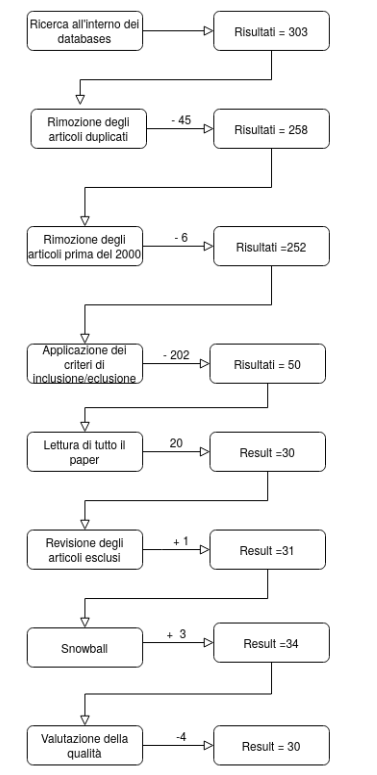
\includegraphics[width=0.4\textwidth]{figura1.5}
	\caption{\emph{Sintesi della selezione degli articoli}}
	\label{fig:fig.2.1}
\end{figure}
\subsection{Minacce alla validità}
\subsubsection{Minaccia alla validità descrittiva}
La validità descrittiva è la misura con cui le osservazioni sono descritte in maniera accurata ed oggettiva. Questo tipo di minaccia è solitamente maggiore negli studi di tipo qualitativo rispetto a quelli di tipo quantitativo. Questa minaccia quindi viene considerata sotto controllo.
\subsubsection{Minaccia alla validità teorica}
La validità teorica è data dalla capacità dell’autore che ha effettuato il mapping study di “cogliere” quello che gli autori degli articoli volevano effettivamente dimostrare. Il fattore che gioca un ruolo fondamentale all’interno di questa minaccia è il pregiudizio che si può avere su determinati autori che a loro
volta influenzano gli articoli da analizzare.

Un'altra minaccia alla validità teorica può derivare dalla formulazione delle
query che potrebbero aver portato a non includere alcuni risultati importanti ai fini dello studio.

Per mitigare questa minaccia si è deciso di applicare la tecnica dello
\emph{snowballing} su tutti gli articoli che sono stati selezionati durante la fase di analisi.
La tecnica ha infatti il fine di individuare artefatti utili che possono essere stati non considerati durante la fase di ricerca.

Infine, la fase di estrazione dei dati effettuata da un singolo ricercatore potrebbe aver portato a non considerare studi importanti. Per mitigare questa minaccia è stato chiesto ad esperto del dominio applicativo ma esterno alla ricerca
di valutare eventuali studi ritenuti dal primo autore “poco chiari”.
\subsubsection{Generalizzazione}
\textbf{Petersen et al}. effettuano una distinzione tra la generalizzazione esterna ed interna. Con la prima si intende la generalizzazione tra gruppi o organizzazioni, mentre con la seconda si indica la generalizzazione all’interno di un singolo gruppo.
I risultati ottenuti potrebbero non essere applicabili all’interno di una revisione sistematica della letteratura poiché gli obiettivi delle ricerche sono differenti.

Tuttavia, visto che si è seguito un approccio di tipo sistematico, gran parte delle
strategie di ricerca risulta in comune, pertanto questa minaccia si ritiene mitigata.
\subsubsection{Validità di interpretazione}
La validità di interpretazione viene raggiunta quando le conclusioni che sono state tratte dai dati risultano essere ragionevoli. Una delle minacce di interpretazione dei dati può essere dovuta al pregiudizio che l’autore del mapping ha verso alcune conclusioni che sono state mostrate nei differenti artefatti. Per mitigare tale minaccia è stato chiesto ad un esperto del dominio applicativo ma esterno alla ricerca di dare un parere sulla veridicità dei dati presi in esame.
\subsubsection{Ripetibilità}
È stato effettuato un mapping study sistematico proprio al fine di garantire la ripetibilità di tutto ciò che si è fatto. Sono state inoltre seguite le linee guida dettate
da \textbf{Kai Petersen, Sairam Vakkalanka et al}. all’interno dell’articolo “\emph{Guidelines
for conducting systematic mapping studies in software engineering: An update}”.

Sono inoltre dettagliate tutte le fasi seguite con assoluto rigore, pertanto tale minaccia risulta mitigata.
\subsection{Analisi dei dati e classificazione}
L’obiettivo dell’analisi dei dati e della classificazione è anche quello di organizzare a livello visivo le informazioni estratte dalle varie domande di ricerca,
in modo che esse possano essere rapidamente individuate e comprese. Le informazioni su ogni articolo sono state mappate ed illustrate visivamente attraverso l’utilizzo di grafici e diagrammi. Successivamente è stato assegnato una categoria ad ogni artefatto e si è passati quindi alla fase di conteggio.
\subsubsection{Numero di dataset (RQ1)}
Dalla prima domanda di ricerca è emerso che in quasi tutti gli studi non è
stato rilasciato un dataset.

Gli unici dataset che sono stati rilasciati (in totale quattro) rientrano nel periodo 2018-2019; questo dato è indice di un argomento di ricerca poco conosciuto e che necessita di ulteriori sviluppi.

Il grafico in figura \ref{fig:fig.2.2} mostra la frequenza di pubblicazione dei dataset messi a disposizione.
\begin{figure}[h]
	\centering
	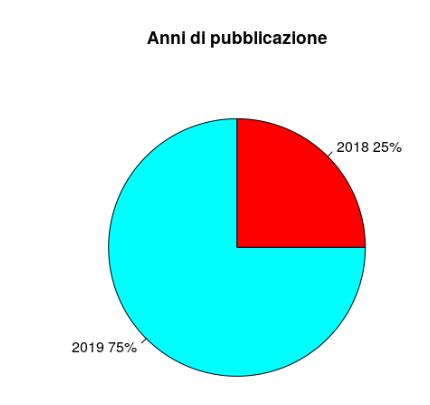
\includegraphics[width=0.7\textwidth]{1.6}
	\caption{\emph{Frequenza di pubblicazione del dataset}}
	\label{fig:fig.2.2}
\end{figure}

Dal grafico è emerso che quasi la totalità dei dataset messi a disposizione
sono stati implementati nel corso del 2019 (75\%). Il numero dei dataset risulta essere comunque molto esiguo.
\subsubsection{Lavoro su progetti closed source (RQ2)}
Dalla seconda domanda di ricerca è emerso che la quasi totalità degli studi effettuati non ha considerato progetti closed-source nella loro valutazione e in alcuni articoli questa problematica è stata considerata solo come minaccia per la validità.

Il grafico in figura \ref{fig:fig2.3} mostra il numero di studi sui quali sono state effettuate ricerche anche su progetti closed-source suddivisi per anno.
\begin{figure}[h]
	\centering
	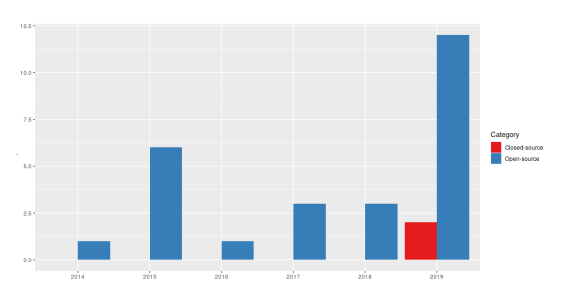
\includegraphics[width=1\textwidth]{2.3}
	\caption{\emph{Numero di progetti su cui sono stati condotti gli studi}}
	\label{fig:fig2.3}
\end{figure}
\subsubsection{Linguaggi di programmazione utilizzati (RQ3)}
Dall'analisi effettuata risulta che quasi tutti gli articoli analizzati riportano le caratteristiche del linguaggio di programmazione impiegato per definire gli oggetti
sperimentali (ventiquattro su trenta). Di questi, quasi la totalità dei progetti
analizzati è scritta in Java (viene infatti definita come una minaccia in alcuni degli
articoli analizzati, in quanto il linguaggio potrebbe presentare alcune caratteristiche
non comuni a tutti i linguaggi di programmazione). È stata quindi approfondita la problematica per capire quale fosse la distribuzione dei linguaggi di programmazione.

Il grafico in figura \ref{2.4} mostra la frequenza di ogni linguaggio di programmazione.
\begin{figure}[h]
	\centering
	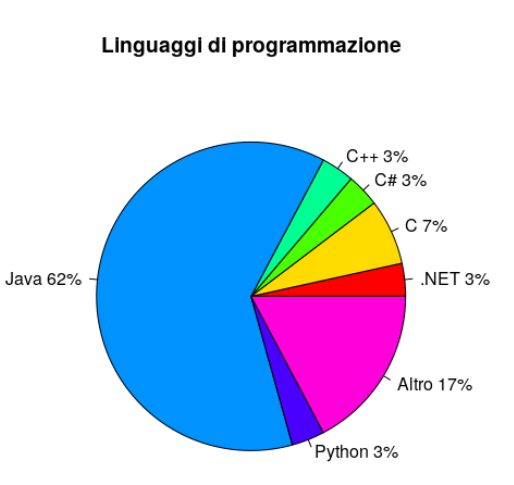
\includegraphics[width=0.9\textwidth]{2.4}
	\caption{\emph{Distribuzione dei linguaggi di programmazione analizzati}}
	\label{fig:fig.2.4}
\end{figure}

È possibile notare che più della metà dei progetti analizzati sono stati sviluppati in Java. Tale dato non stupisce in quanto attualmente il linguaggio Java risulta essere uno dei più utilizzati al mondo. È altresì importante sottolineare che per alcuni linguaggi la problematica è stata trattata solo in minima parte o non è stata per nulla trattata.
\subsubsection{Tipi di build utilizzati (RQ4)}
Dall’analisi effettuata è emerso che non sempre è stato dichiarato
esplicitamente il sistema di build adoperato durante la costruzione del dataset.

Negli articoli in cui tale informazione è presente, il linguaggio di programmazione utilizzato è sempre stato Java. Dei trenta articoli, in nove è stato riportato anche il tipo di build system utilizzato (in alcuni casi anche più di uno).

Il grafico in figura \ref{fig:fig.2.5} mostra la frequenza dei sistemi di building utilizzati
all’interno dei progetti che sono stati testati.
\begin{figure}[h]
	\centering
	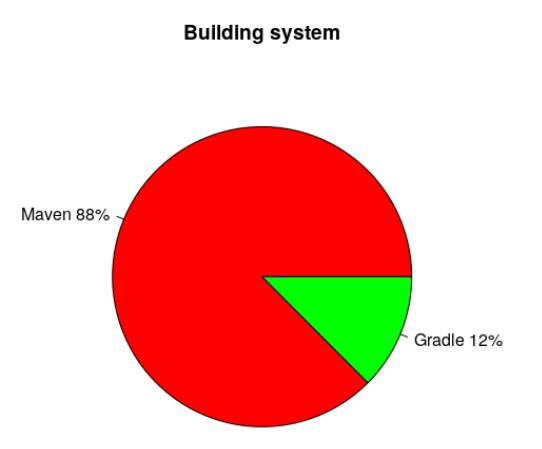
\includegraphics[width=0.6\textwidth]{2.5}
	\caption{\emph{Sistemi di building utilizzati}}
	\label{fig:fig.2.5}
\end{figure}

È possibile notare che quasi la totalità dei progetti analizzati utilizzano come sistema di build Maven (preso in considerazione in sette articoli), mentre solo il 12\% utilizzano Gradle (preso in considerazione in un solo articolo).
\subsubsection{Individuazione del dataset (RQ5)}
In tutti gli articoli in cui è stata dichiarata la costruzione del dataset (diciotto articoli), è stato anche descritto il metodo utilizzato per la descrizione.

La strategia più comune risulta quella di scaricare da GitHub i repository più popolari per poi verificare la presenza di metodi flaky (38\%).

Le altre strategie utilizzate si basano principalmente sull’uso di Travis (valutando lo stato della build oppure i file di log generati) e sul cercare la stringa “flaky” all’interno dei bug report o nei messaggi di commit all’interno del motore di ricerca di GitHub.

Il grafico in figura \ref{fig:fig.2.6} mostra la percentuale di utilizzo di ogni strategia per individuare i dataset.

\begin{figure}[h]
	\centering
	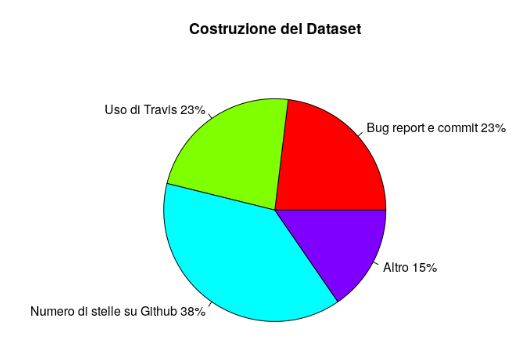
\includegraphics[width=0.6\textwidth]{2.6}
	\caption{\emph{Strategie usate per la costruzione del dataset}}
	\label{fig:fig.2.6}
\end{figure}
\subsubsection{Quali sono le root cause più frequenti (RQ6)}
Sui trenta articoli esaminati solo in dieci casi sono state individuate le \emph{root cause} dei \emph{flaky test}.

In gran parte degli articoli le root cause risultano le stesse,
ossia: dipendenza dall’ordine, concorrenza, async wait, tempo, rete, random, perdita di risorse, operazioni con numeri float e problemi di I/O.

È però interessante soffermarsi sulle root cause “Output restrittivi” e “Interfaccia grafica”, tali root
cause infatti sono presenti con una percentuale molto bassa (2\%) poiché non sono state mai individuate precedentemente, ma sono frutto di studi effettuati nel 2019. 

Possiamo quindi definirle nel seguente modo:
\begin{itemize}
	\item \emph{Output restrittivi}: Sono degli output validi, ma considerati fuori dai “range” consentiti per questioni di design;
	\item \emph{Interfaccia grafica}: Un’interfaccia grafica viene definita come “flaky” nel momento in cui avviene una mancata comunicazione tra il processo che esegue il rendering e l’interfaccia stessa.
\end{itemize}

La figura \ref{fig:fig.2.7} mostra le root cause più comuni.
\newpage
\begin{figure}[h]
	\centering
	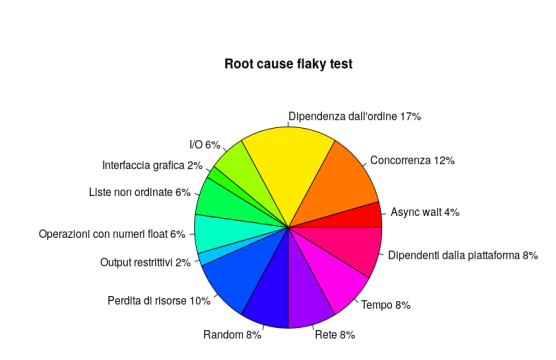
\includegraphics[width=1\textwidth]{2.7}
	\caption{\emph{Root cause dei flaky test}}
	\label{fig:fig.2.7}
\end{figure}
\subsubsection{Metodo empirico per la valutazione delle root cause (RQ7)}
Dagli articoli che rispondono a questa domanda di ricerca sono state estratte le tecniche adoperate per valutare le root cause dei flaky test.

Nel 29\% dei casi, il metodo comunemente utilizzato al momento consiste
nell’effettuare nuovamente l’esecuzione di un caso di test e verificare se quest’ultimo cambia stato rispetto all’esecuzione precedente (pass/fail o viceversa). Le altre strategie adoperate sono:
%AGGIUNGERE BENE I SUBITEM
\begin{itemize}
	\item Strumentazione del codice: Creazione di un codice che monitora comportamenti specifici di una applicazione;
	\item Coverage: Con questa tecnica viene calcolata la coverage (solitamente la line) ogni volta che il caso di test viene eseguito, se si riscontra un cambio di coverage in parti del codice che non sono state modificate, il test viene classificato come flaky;
	\item Analisi del codice: L’analisi del codice può essere eseguita in due modi:
	\subitem Statica: In questo caso gli sviluppatori definiscono un metodo flaky se rilevano che nel codice sorgente del test viene fatto uso di qualche funzione che può generare un flaky;
	\subitem Dinamica: Viene eseguito il codice sorgente del test e si valutano glioutput generati e i file di log scritti. Se si nota una discordanza tra le due esecuzioni, il metodo viene definito flaky.
\end{itemize}

Il grafico in figura \ref{fig:fig.2.8} mostra le frequenze di utilizzo di ogni tecnica che è stata descritta precedentemente.
\newpage
\begin{figure}[h]
	\centering
	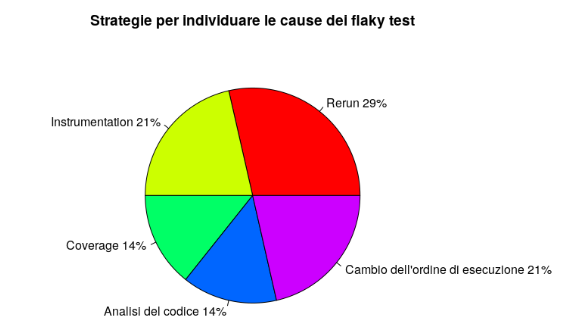
\includegraphics[width=1\textwidth]{2.8}
	\caption{\emph{Strategia per individuare i flaky test}}
	\label{fig:fig.2.8}
\end{figure}
\subsubsection{A chi viene indirizzata la ricerca mostrata nei diversi studi (RQ8)}
Dall'analisi effettuata è emerso che in cinque artefatti è chiaramente indicato a chi fosse rivolto lo studio (grandi aziende e ambito accademico); invece, nei restanti artefatti si può intuire che lo studio è rivolto ad un pubblico prettamente accademico.

La figura \ref{fig:fig.2.9} mostra la percentuale degli articoli dove vengono menzionati sia le aziende che gli accademici come fruitori finali dello studio, comparato a quelli dove vengono citati solo gli accademici.\newpage
\begin{figure}[h]
	\centering
	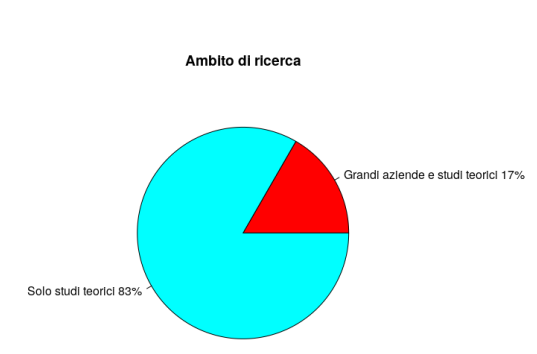
\includegraphics[width=1\textwidth]{2.9}
	\caption{\emph{Ambito di ricerca per ogni artefatto}}
	\label{fig:fig.2.9}
\end{figure}

È interessante soffermarsi su quest’ultima percentuale poiché nonostante il problema sia stato posto inizialmente dalle grandi aziende (Google, Facebook, Huawei in primis), esso è diventato un argomento su cui sono nati molteplici studi da parte degli accademici.
\subsubsection{Anno di pubblicazione (RQ9)}
Gran parte degli studi sono stati pubblicati tra il 2018 e il 2019 (il 63\%), questo ci suggerisce che l’argomento rappresenta una problematica attuale ed è tuttora molto studiato.
La figura \ref{fig:fig.2.10} mostra la frequenza di pubblicazione degli artefatti suddivisa per anni.
\newpage
\begin{figure}[h]
	\centering
	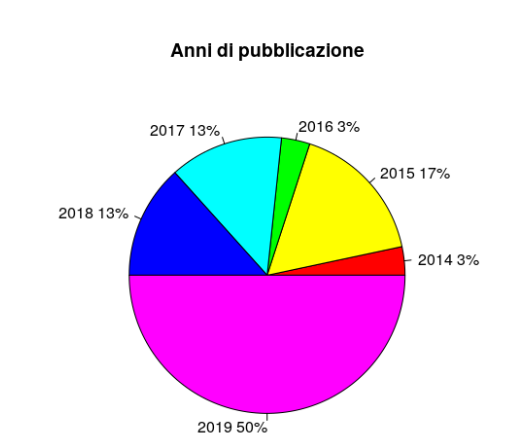
\includegraphics[width=1\textwidth]{2.10}
	\caption{\emph{Frequenza di pubblicazione suddivisa per anni}}
	\label{fig:fig.2.10}
\end{figure}
\subsection{Conclusioni}
	Dallo studio effettuato è emerso che:
\begin{itemize}

	\item  Gli unici studi sui quali sono stati effettivamente rilasciati dei dataset sono
	solo quelli presentati tra il 2018 e il 2019, tale dato ci porta a sottolineare l’importanza e la necessità da parte sia delle aziende che degli accademici
	di rilasciare nuovi dati o di ampliare quelli già esistenti;
	\item Bisogna analizzare con particolare attenzione anche progetti closed-source
	poiché le dinamiche e i meccanismi con cui vengono costruiti tali progetti possono essere completamente differenti da quelle open-source;
	\item Occorre prestare maggiore attenzione anche ad altri tipi di linguaggi di programmazione, poiché gran parte degli studi sono stati effettuati soltanto
	su progetti scritti in Java e che utilizzano Maven come build system;
	\item  L’uso di GitHub per individuare progetti open-source affetti da flakiness è effettivamente un buon punto di partenza ma bisognerebbe analizzare anche
	repository private o progetti closed-source;
	\item  Negli anni le root cause individuate sono state ampliate per comprendere nuove piattaforme mai considerate in precedenza (es. Android); tale
	ampliamento ha permesso di considerare all’interno delle root cause anche problemi legati all’hardware (es. fotocamera non disponibile). Attualmente questi problemi sono ancora classificati all’interno della causa “problemi
	dipendenti dalla piattaforma”, ma non si esclude che possano diventare una nuova categoria in futuro.
\end{itemize}
